\documentclass[journal,12pt,twocolumn]{IEEEtran}

\usepackage{setspace}
\usepackage{gensymb}
\singlespacing
\usepackage[cmex10]{amsmath}

\usepackage{amsthm}
\usepackage{amsmath,amssymb}
\usepackage{mathrsfs}
\usepackage{txfonts}
\usepackage{stfloats}
\usepackage{bm}
\usepackage{cite}
\usepackage{cases}
\usepackage{subfig}

\usepackage{longtable}
\usepackage{multirow}
\usepackage{float}
\usepackage{enumitem}
\usepackage{mathtools}
\usepackage{steinmetz}
\usepackage{tikz}
\usepackage{circuitikz}
\usepackage{verbatim}
%\usepackage{tfrupee}
\usepackage[breaklinks=true]{hyperref}
\usepackage{graphicx}
\usepackage{tkz-euclide}
\usepackage{stackengine}
\usetikzlibrary{calc,math}
\usepackage{listings}
    \usepackage{color}                                            %%
    \usepackage{array}                                            %%
    \usepackage{longtable}                                        %%
    \usepackage{calc}                                             %%
    \usepackage{multirow}                                         %%
    \usepackage{hhline}                                           %%
    \usepackage{ifthen}                                           %%
    \usepackage{lscape}     
\usepackage{multicol}
\usepackage{chngcntr}
\usepackage{bm}
\DeclareMathOperator*{\Res}{Res}

\renewcommand\thesection{\arabic{section}}
\renewcommand\thesubsection{\thesection.\arabic{subsection}}
\renewcommand\thesubsubsection{\thesubsection.\arabic{subsubsection}}

\renewcommand\thesectiondis{\arabic{section}}
\renewcommand\thesubsectiondis{\thesectiondis.\arabic{subsection}}
\renewcommand\thesubsubsectiondis{\thesubsectiondis.\arabic{subsubsection}}


\hyphenation{op-tical net-works semi-conduc-tor}
\def\inputGnumericTable{}                                 %%

\lstset{
%language=C,
frame=single, 
breaklines=true,
columns=fullflexible
}
\makeatletter
\setlength{\@fptop}{0pt}
\makeatother
\begin{document}

\newtheorem{theorem}{Theorem}[section]
\newtheorem{problem}{Problem}
\newtheorem{proposition}{Proposition}[section]
\newtheorem{lemma}{Lemma}[section]
\newtheorem{corollary}[theorem]{Corollary}
\newtheorem{example}{Example}[section]
\newtheorem{definition}[problem]{Definition}

\newcommand{\BEQA}{\begin{eqnarray}}
\newcommand{\EEQA}{\end{eqnarray}}
\newcommand{\define}{\stackrel{\triangle}{=}}
\bibliographystyle{IEEEtran}
\raggedbottom
\setlength{\parindent}{0pt}
\providecommand{\mbf}{\mathbf}
\providecommand{\pr}[1]{\ensuremath{\Pr\left(#1\right)}}
\providecommand{\qfunc}[1]{\ensuremath{Q\left(#1\right)}}
\providecommand{\sbrak}[1]{\ensuremath{{}\left[#1\right]}}
\providecommand{\lsbrak}[1]{\ensuremath{{}\left[#1\right.}}
\providecommand{\rsbrak}[1]{\ensuremath{{}\left.#1\right]}}
\providecommand{\brak}[1]{\ensuremath{\left(#1\right)}}
\providecommand{\lbrak}[1]{\ensuremath{\left(#1\right.}}
\providecommand{\rbrak}[1]{\ensuremath{\left.#1\right)}}
\providecommand{\cbrak}[1]{\ensuremath{\left\{#1\right\}}}
\providecommand{\lcbrak}[1]{\ensuremath{\left\{#1\right.}}
\providecommand{\rcbrak}[1]{\ensuremath{\left.#1\right\}}}
\DeclarePairedDelimiter\ceil{\lceil}{\rceil}
\DeclarePairedDelimiter\floor{\lfloor}{\rfloor}
\theoremstyle{remark}
\newtheorem{rem}{Remark}
\newcommand{\sgn}{\mathop{\mathrm{sgn}}}
\providecommand{\abs}[1]{\vert#1\vert}
\providecommand{\res}[1]{\Res\displaylimits_{#1}} 
\providecommand{\norm}[1]{\lVert#1\rVert}
%\providecommand{\norm}[1]{\lVert#1\rVert}
\providecommand{\mtx}[1]{\mathbf{#1}}
\providecommand{\mean}[1]{E[ #1 ]}
\providecommand{\fourier}{\overset{\mathcal{F}}{ \rightleftharpoons}}
%\providecommand{\hilbert}{\overset{\mathcal{H}}{ \rightleftharpoons}}
\providecommand{\system}{\overset{\mathcal{H}}{ \longleftrightarrow}}
	%\newcommand{\solution}[2]{\textbf{Solution:}{#1}}
\newcommand{\solution}{\noindent \textbf{Solution: }}
\newcommand{\cosec}{\,\text{cosec}\,}
\newcommand*{\permcomb}[4][0mu]{{{}^{#3}\mkern#1#2_{#4}}}
\newcommand*{\perm}[1][-3mu]{\permcomb[#1]{P}}
\newcommand*{\comb}[1][-1mu]{\permcomb[#1]{C}}
\newcommand\xrowht[2][0]{\addstackgap[.5\dimexpr#2\relax]{\vphantom{#1}}}
\providecommand{\dec}[2]{\ensuremath{\overset{#1}{\underset{#2}{\gtrless}}}}
\newcommand{\myvec}[1]{\ensuremath{\begin{pmatrix}#1\end{pmatrix}}}
\newcommand{\mydet}[1]{\ensuremath{\begin{vmatrix}#1\end{vmatrix}}}
\numberwithin{equation}{subsection}
\makeatletter
\@addtoreset{figure}{problem}
\makeatother
\let\StandardTheFigure\thefigure
\let\vec\mathbf
\renewcommand{\thefigure}{\theproblem}
\def\putbox#1#2#3{\makebox[0in][l]{\makebox[#1][l]{}\raisebox{\baselineskip}[0in][0in]{\raisebox{#2}[0in][0in]{#3}}}}
     \def\rightbox#1{\makebox[0in][r]{#1}}
     \def\centbox#1{\makebox[0in]{#1}}
     \def\topbox#1{\raisebox{-\baselineskip}[0in][0in]{#1}}
     \def\midbox#1{\raisebox{-0.5\baselineskip}[0in][0in]{#1}}
\vspace{3cm}
\title{Gate Assignment - 2}
\author{Chirag Mehta - AI20BTECH11006}
\maketitle
\newpage
\bigskip
\renewcommand{\thefigure}{\theenumi}
\renewcommand{\thetable}{\theenumi}
Download all the python codes from
\begin{lstlisting}
https://github.com/cmaspi/EE3900/tree/main/GateAssignment-2/code
\end{lstlisting}
latex-tikz codes from 
\begin{lstlisting}
https://github.com/cmaspi/EE3900/blob/main/GateAssignment-2/main.tex
\end{lstlisting}
\section{Problem}
(GATE EC 2009 Q42)
The 4-point discrete fourier transform (DFT) of a discrete time sequence $[1,0,2,3]$ is given by
\begin{enumerate}
    \item $[0,-2+2j,2,-2-2j]$
    \item $[2,2+j,6,2-2j]$
    \item $[6,1-3j,2,1+3j]$
    \item $[6,-1+3j,0,-1,-3j]$
\end{enumerate}
\section{Solution}
% \begin{lemma}
%     The N-point discrete fourier transform is given as $\vec{X}=\vec{Wx}$, where $\vec{x}$ is the input signal, $\vec{W}$ is the N-by-N square DFT matrix, and $\vec{X}$ is the DFT of the signal.\\
%     The transformation matrix $\vec{W}$ is given by
%     \begin{align}
%         \vec{W}=\myvec{1 & 1 & \dots & 1 \\ 1 & w & \dots & w^{N-1} \\ \vdots & \vdots & \ddots & \vdots\\ 1 & w^{N-1} & \dots & w^{(N-1)(N-1)}}
%     \end{align}
%     where $w=e^{\frac{-2\pi j}{N}}$
% \end{lemma}

% The four point DFT matrix is given below
% \begin{align}
%     W=\myvec{1 & 1 & 1 & 1\\ 1 & -j & -1 & j \\ 1 & -1 & 1 & -1 \\ 1 & j & -1 & -j}
% \end{align}
% Now,
% \begin{align}
%     \vec{X}=\vec{Wx}
% \end{align}
% On multiplying, we get 
% \begin{align}
%     X=\myvec{6\\-1+3j\\0\\-1-3j}
% \end{align}
% The correct answer is \textbf{option D}
The discrete input signal is
\begin{align}
    x(n)=[1,0,2,3]
\end{align}
Let $\vec{F}_N$ be the N-point DFT matrix.\\
Using the property of complex exponentials, we can express $\vec{F}_N$ in terms of $\vec{F}_{N/2}$
\begin{align}
    \vec{F}_N=\myvec{\vec{I}_{N/2} & \vec{D}_{N/2} \\ \vec{I}_{N/2} & -\vec{D}_{N/2}}\myvec{\vec{F}_{N/2} & \vec{0} \\ \vec{0} & \vec{F}_{N/2}}\vec{P}_N
\end{align}
Where
\begin{align}
    \vec{F}_N=\myvec{1 & 1 & \cdots & 1 \\ 1 & w & \cdots & w^{N-1} \\ \vdots & \vdots & \ddots & \vdots\\ 1 & w^{N-1} & \cdots & w^{(N-1)(N-1)}}
\end{align}
where $w=e^{\frac{-2\pi j}{N}}$
\begin{align}
\vec{D}_N=\myvec{w_{2N}^0 & 0 & \cdots\\ 0 & w_{2N}^1 &  \cdots \\ \vdots & \vdots & \ddots }\\
\vec{D}_N=\text{diag}(w_{2N}^0,w_{2N}^1,\ldots,w_{2N}^{N-1})
\end{align}
$P_{2N}$ is the permutation matrix defined as 
\begin{align}
    \vec{P}_N&=\sbrak{a_{ij}}_{N\times N},\, i,j\in\cbrak{0,1,\ldots,N-1}\\
	a_{ij} &=
\begin{cases}
1 & j=2i,\, i<\frac{N}{2}\\
1 &  j=2\brak{i-\frac{N}{2}}+1,\, i\geq \frac{N}{2}\\
0 & otherwise
\end{cases}
\label{eq:final_result}
\end{align}

For $N=4$
\begin{align}
    \vec{F}_4=\myvec{\vec{I}_2 & \vec{D}_{2} \\ \vec{I}_{2} & -\vec{D}_{2}}\myvec{\vec{F}_{2} & \vec{0} \\ \vec{0} & \vec{F}_{2}}\vec{P}_4
\end{align}
$I_{2}$ is $2\times 2$ matrix
\begin{align}
    \vec{D}_2 & =\myvec{w_4^0 & 0\\0 & w_4^1}\\
    \vec{P}_4 & =\myvec{1&0&0&0\\0&0&1&0\\0&1&0&0\\0&0&0&1}
\end{align}
Now,
\begin{align}
    \myvec{X(0)\\X(1)}&=\myvec{X_e(0)\\X_e(1)}+\vec{D}_2\myvec{X_o(0)\\X_o(1)}\\
    \myvec{X(2)\\X(3)}&=\myvec{X_e(0)\\X_e(1)}-\vec{D}_2\myvec{X_o(0)\\X_o(1)}
\end{align}
This results in
\begin{align}
    \myvec{X(0)\\X(1)} & =\vec{F}_2\myvec{1\\2}+\myvec{1&0\\0&-j}\vec{F}_2\myvec{0\\3}\\    
    \myvec{X(0)\\X(1)} & =\myvec{3\\-1}+\myvec{3\\3j}\\
    \myvec{X(0)\\X(1)} & =\myvec{6\\-1+3j}
\end{align}
and
\begin{align}
    \myvec{X(2)\\X(3)}&=\vec{F}_2\myvec{1\\2}-\myvec{1&0\\0&-j}\vec{F}_2\myvec{0\\3}\\    
    \myvec{X(2)\\X(3)}&=\myvec{3\\-1}-\myvec{3\\3j}\\
    \myvec{X(2)\\X(3)}&=\myvec{0\\-1-3j}
\end{align}
The correct answer is \textbf{option 4}
\begin{figure}[!ht]
    \centering
    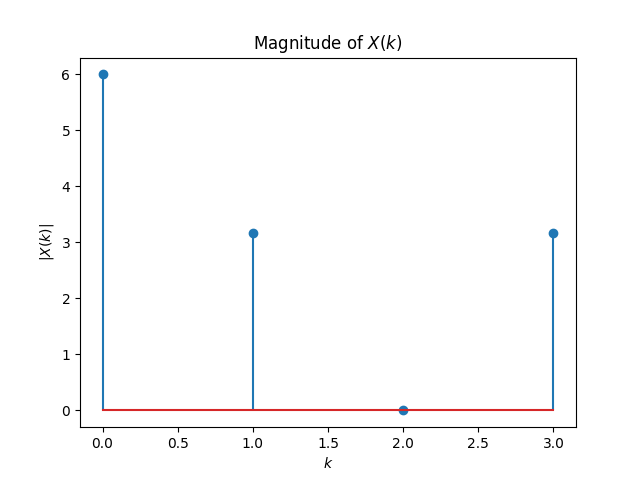
\includegraphics[width=\columnwidth]{plot/magnitude}
    \caption{Magnitude of $X(k)$}
    \label{magnitude}
\end{figure}
\begin{figure}[!ht]
    \centering
    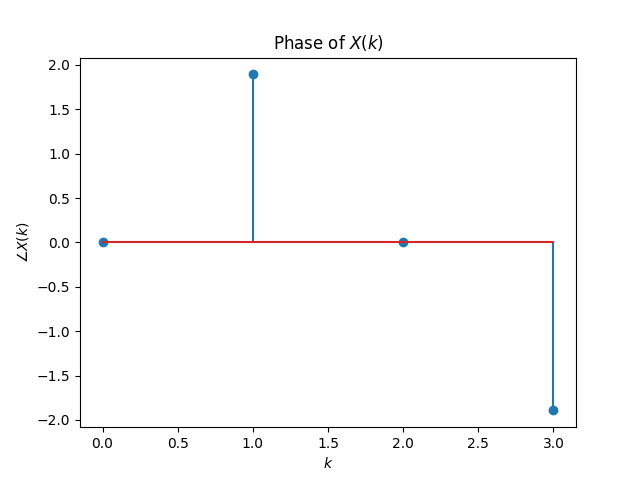
\includegraphics[width=\columnwidth]{plot/phase}
    \caption{Phase of $X(k)$}
    \label{magnitude}
\end{figure}
\end{document}